\documentclass[11pt]{beamer}

\usetheme{Singapore}
\usepackage[utf8]{inputenc}
\usepackage{amsmath}
\usepackage{amsfonts}
\usepackage{amssymb}
\usepackage{graphicx}
\usepackage{hyperref}
\usepackage{setspace}
\usepackage{booktabs}
\usepackage{listings}
\usepackage{xcolor}
\usepackage{caption}
\usepackage{subcaption}

% Set line spacing
\let\oldframetitle\frametitle% Store old \frametitle in \oldframetitle
\renewcommand{\frametitle}[1]{% Redefine \frametitle
  \oldframetitle{#1}\setstretch{1.3}}


% Define the settings for codechunks
\definecolor{codegreen}{rgb}{0,0.6,0}
\definecolor{codegray}{rgb}{0.5,0.5,0.5}
\definecolor{codepurple}{rgb}{0.58,0,0.82}
\definecolor{backcolour}{rgb}{0.9,0.9,0.9}
\lstdefinestyle{mystyle}{
    backgroundcolor=\color{backcolour},   
    commentstyle=\color{codegreen},
    keywordstyle=\color{magenta},
    numberstyle=\tiny\color{codegray},
    stringstyle=\color{codepurple},
    basicstyle=\ttfamily\footnotesize,
    breakatwhitespace=false,         
    breaklines=true,                 
    captionpos=b,                    
    keepspaces=true,                 
    numbers=left,                    
    numbersep=5pt,                  
    showspaces=false,                
    showstringspaces=false,
    showtabs=false,                  
    tabsize=2
}
\lstset{style=mystyle}

% Setup the bibliography
\usepackage[style=authortitle,backend=bibtex,citestyle=authortitle]{biblatex}
\addbibresource{../bibliography.bib}
\setbeamertemplate{bibliography item}[text]
\setbeamerfont{footnote}{size=\tiny}

% Allow footnotes with no number
\newcommand\blfootnote[1]{%
  \begingroup
  \renewcommand\thefootnote{}\footnote{#1}%
  \addtocounter{footnote}{-1}%
  \endgroup
}

% Allow section title slides
\AtBeginSection[]{
  \begin{frame}
  \vfill
  \centering
  \begin{beamercolorbox}[sep=8pt,center,shadow=true,rounded=true]{title}
    \usebeamerfont{title}\insertsectionhead\par%
  \end{beamercolorbox}
  \vfill
  \end{frame}
}

\author{Stephen Pederson}
\title{DRMCRL}
\subtitle{Group Meeting}
\setbeamercovered{transparent} 
\setbeamertemplate{navigation symbols}{} 
\logo{
	
\includegraphics[scale=0.25]{../images/UoA_logo_col_vert.png} 
	\hspace{0.84\linewidth}
	
\includegraphics[scale=0.06]{../images/DRMCRL_BANNER_3lines.png} 
} 
\institute{Dame Roma Mitchell Cancer Research Laboratories, \\The University of Adelaide} 
\date{25\textsuperscript{th} August, 2020} 


\begin{document}

\begin{frame}
\titlepage
\end{frame}

\begin{frame}
\footnotesize
\tableofcontents
\end{frame}

\section{Introduction}

\begin{frame}{Bioinformatics Hub}

	\begin{itemize}
		\item Co-ordinator Bioinformatics Hub, 2014 - 2020
		\item Currently an ECR: PhD (2008-2018)
		\item Main areas of expertise:
		\begin{itemize}
			\item \texttt{R}, \texttt{bash}, \LaTeX
			\item Transcriptomics and Statistics
		\end{itemize}
	\end{itemize}

\end{frame}

\subsection{Why such a long PhD?}

\begin{frame}{Why such a long PhD?}

	\begin{itemize}
		\item Detect alternate transcript usage using whole-transcript microarrays
		\item Built a Bayesian model which ran a MCMC process (written in C)
		\item Implemented as an R package 
	\end{itemize}

\end{frame}

\begin{frame}{Why such a long PhD?}

	\begin{itemize}
		\item Pre-RStudio, Pre-\texttt{tidyverse}, Pre-\texttt{RMarkdown}, Pre-\texttt{Rcpp}
		\item Model significantly ``under-performed" on real data
		\item Broke the software with no version control strategy 
		\begin{itemize}
			\item MCMC process ran for a week on 4-cores 
			\item Failure was a random failure to complete (probably C memory issues)
			\item Took 6 months to debug
		\end{itemize}
		\item \textit{No bioinformatics community able to help}
	\end{itemize}

\end{frame}

\begin{frame}{Why such a long PhD?}

	\begin{itemize}
		\item Tutored for School of Mathematical Sciences
		\item Picked up large amounts of work as a musician
		\item Landlord died $\implies$ no place to live
		\item Bioinfosummer 2013 (Terry Speed)
	\end{itemize}

\end{frame}

\subsection{The Bioinformatics Hub}

\begin{frame}{Formation of the Bioinformatics Hub}

An application was made to the IDRF

\small

	\begin{enumerate}
		\item Prof David Adelson: Head, School of Biological Sciences; Chair of Bioinformatics
		\item Prof Gary Glonek: Head, School of Mathematical Sciences
		\item Prof Mike Wilkinson: Head, School of Agriculture, Food \& Wine
		\item Prof Julie Owen: Head, School of Paediatrics \& Reproductive Health
	\end{enumerate}
	
Others named with a key interest: \textit{Prof Alan Cooper, Prof Wayne Tilley, Prof Sarah Robertson etc}\\[5mm]

\end{frame}

\begin{frame}{Formation of the Bioinformatics Hub}

	\begin{itemize}
		\item Run training workshops, seminars, journal clubs etc
		\item Manage a hot-desking facility
		\item Provide consultations and advice
		\item Develop formal courses and subjects
		\item Apply for external research funding
		\item Build a \textit{critical mass}
	\end{itemize}
	
	Interestingly, this is not a core-facility\\[5mm]

\end{frame}

\begin{frame}{Formation of the Bioinformatics Hub}

	\begin{itemize}
		\item Directors: 
		\begin{itemize}
			\item 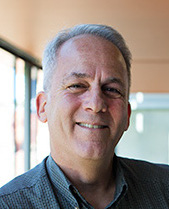
\includegraphics[height=1cm]{figures/dave.jpg} David Adelson (\textit{Biol. Sci.})
			\item 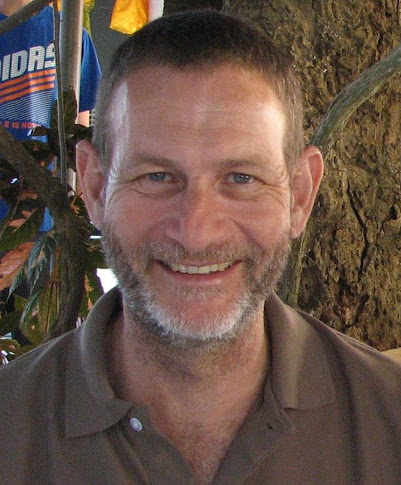
\includegraphics[height=1cm]{figures/gary.jpg} Gary Glonek (\textit{Mathematical Sciences})
		\end{itemize}			
		\item Funded by DVCR to recruit Level B6-C3 Academic for 2014 
		\item Administered within School of Biological Sciences (BS)\\[1cm]

	\end{itemize}	
	
\end{frame}

\begin{frame}{Formation of the Bioinformatics Hub}
	
	\begin{itemize}
		\item I commenced in March 2014: 10 month contract at Level A4
	\end{itemize}
	
	Why?

	\begin{itemize}
		\item Not attractive for external recruitment
		\item Unemployed bioinformaticians are unicorns
		\item I was the ``best they could get"\\[2cm]
	\end{itemize}
	
\end{frame}

\begin{frame}{2015}

	\begin{itemize}
		\item My contract was renewed for 2015
		\item 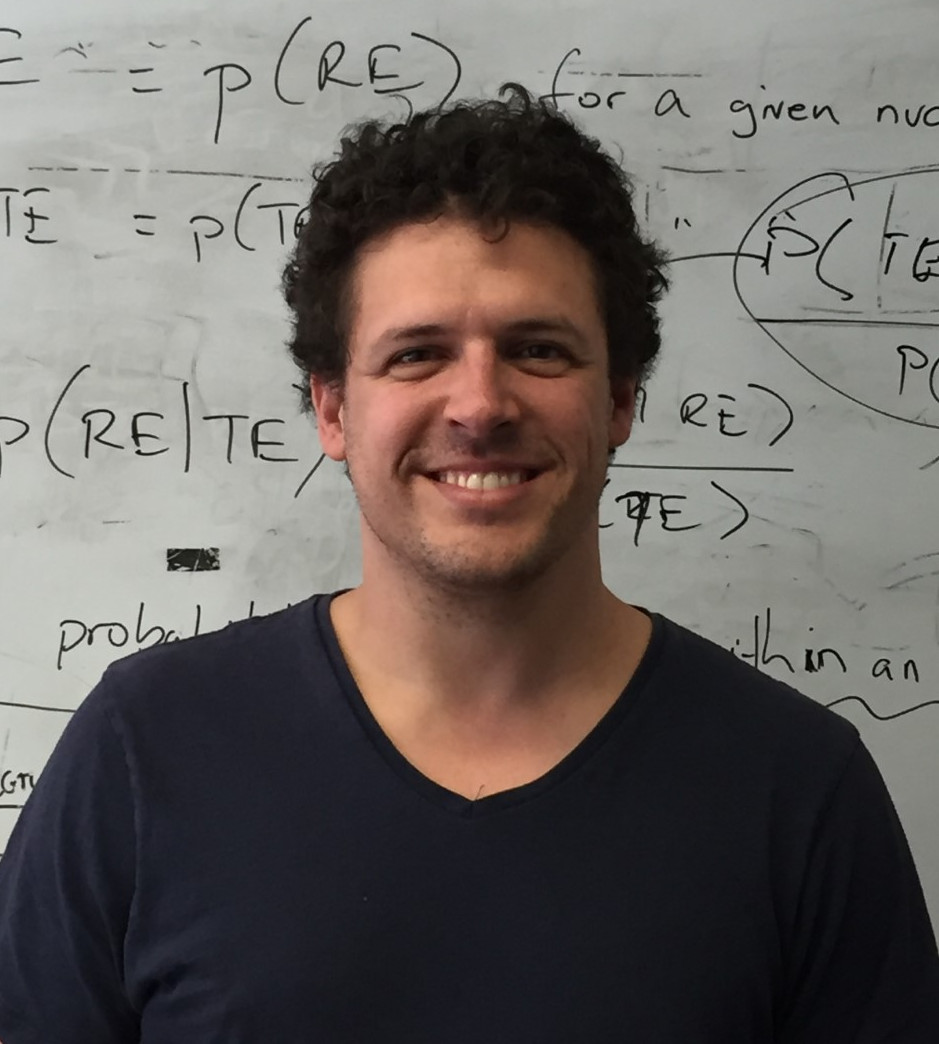
\includegraphics[height=1cm]{figures/Jimmy.jpg} Jimmy Breen appointed to RRI $\implies$ co-located
		\item 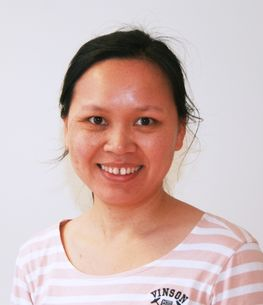
\includegraphics[height=1cm]{figures/hien.jpg} Hien To appointed as second staff member (2015-2018)
		\item 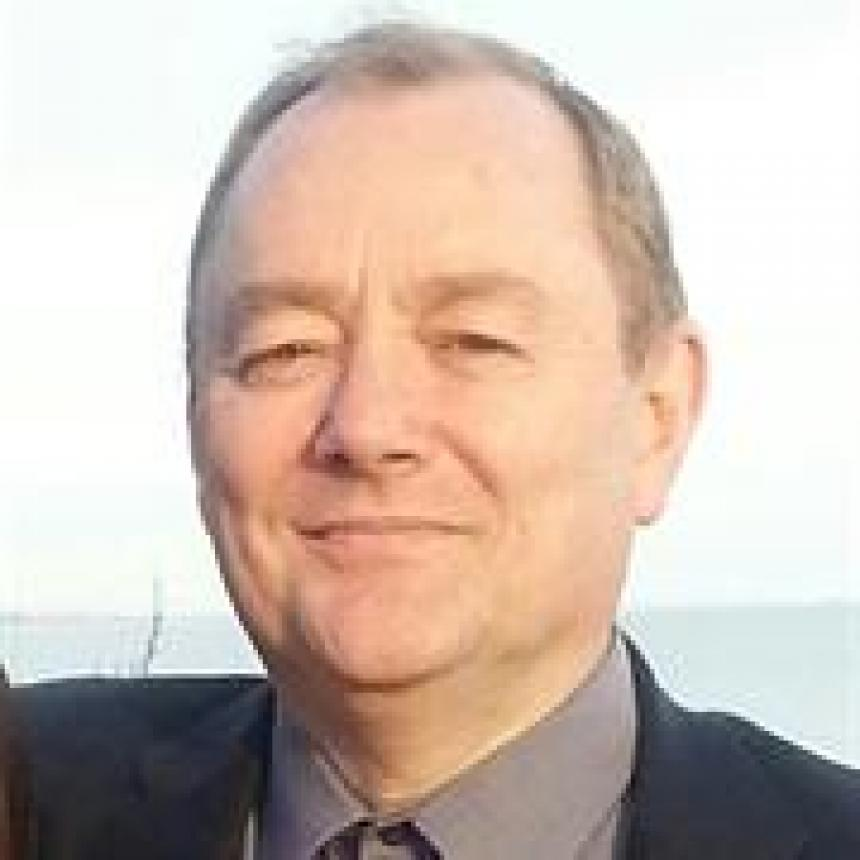
\includegraphics[height=1cm]{figures/rick.jpeg} Rick Tearle appointed to Davies Research Centre (Roseworthy)\\[8mm]
	\end{itemize}		
	
\end{frame}

\begin{frame}{In Later Years}

	\begin{itemize}
		\item 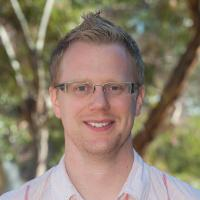
\includegraphics[height=1cm]{figures/Watson-Haigh.jpeg} Nathan Watson-Haigh (2018-2020) 
		\item 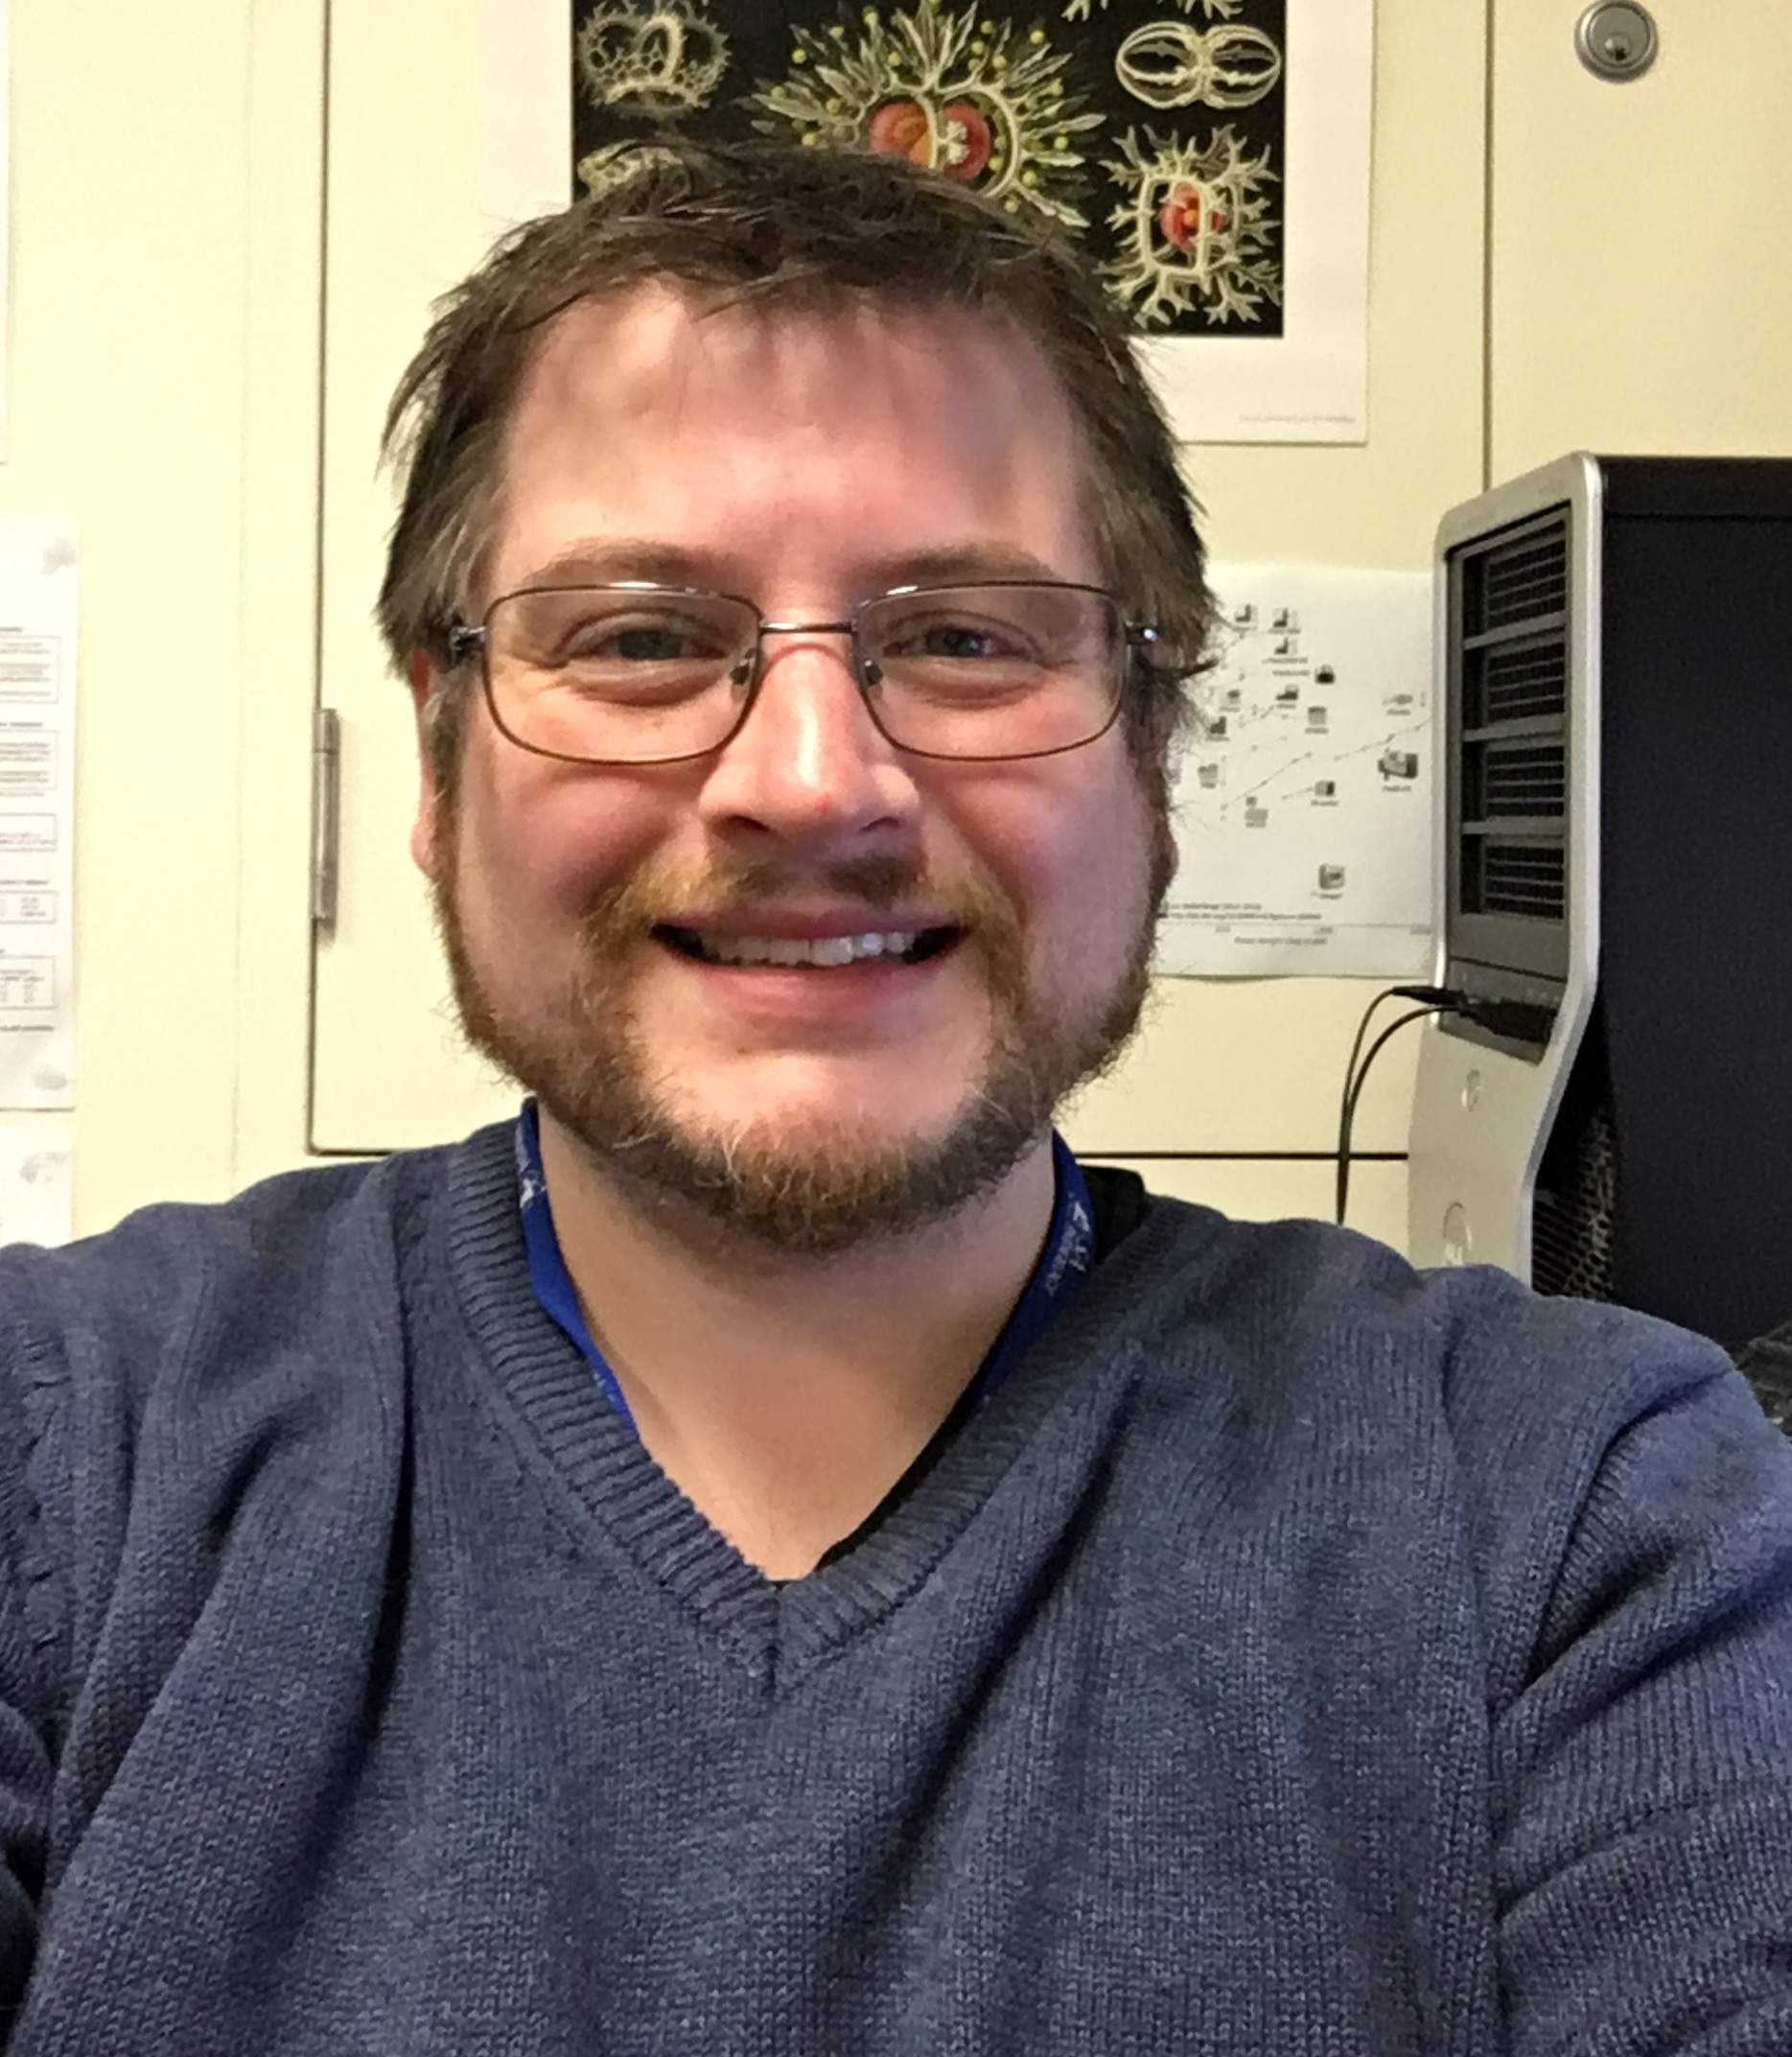
\includegraphics[height=1cm]{figures/Mark.jpg}  Mark Armstrong (2019-2020)
		\item Additional 12 staff members (2015-2020)
	\end{itemize}
	~\\[1cm]
	
\end{frame}


\subsection{Our Track Record}

\begin{frame}{Our Track Record}

Over our existence:

	\begin{itemize}
		\item \$8.5m in grant funding
		\item $>$1400 distinct individuals through workshops
		\item Individual support for $>$360 postgraduate students (MPhil/PhD)
		\item Co-authored 84 publications + 2 software packages
		\item Established a Bioinformatics Undergraduate Major
		\item Very strong and supportive bioinformatics community\\[5mm]
	\end{itemize}

\end{frame}

\begin{frame}{Our Track Record}

\small
\center
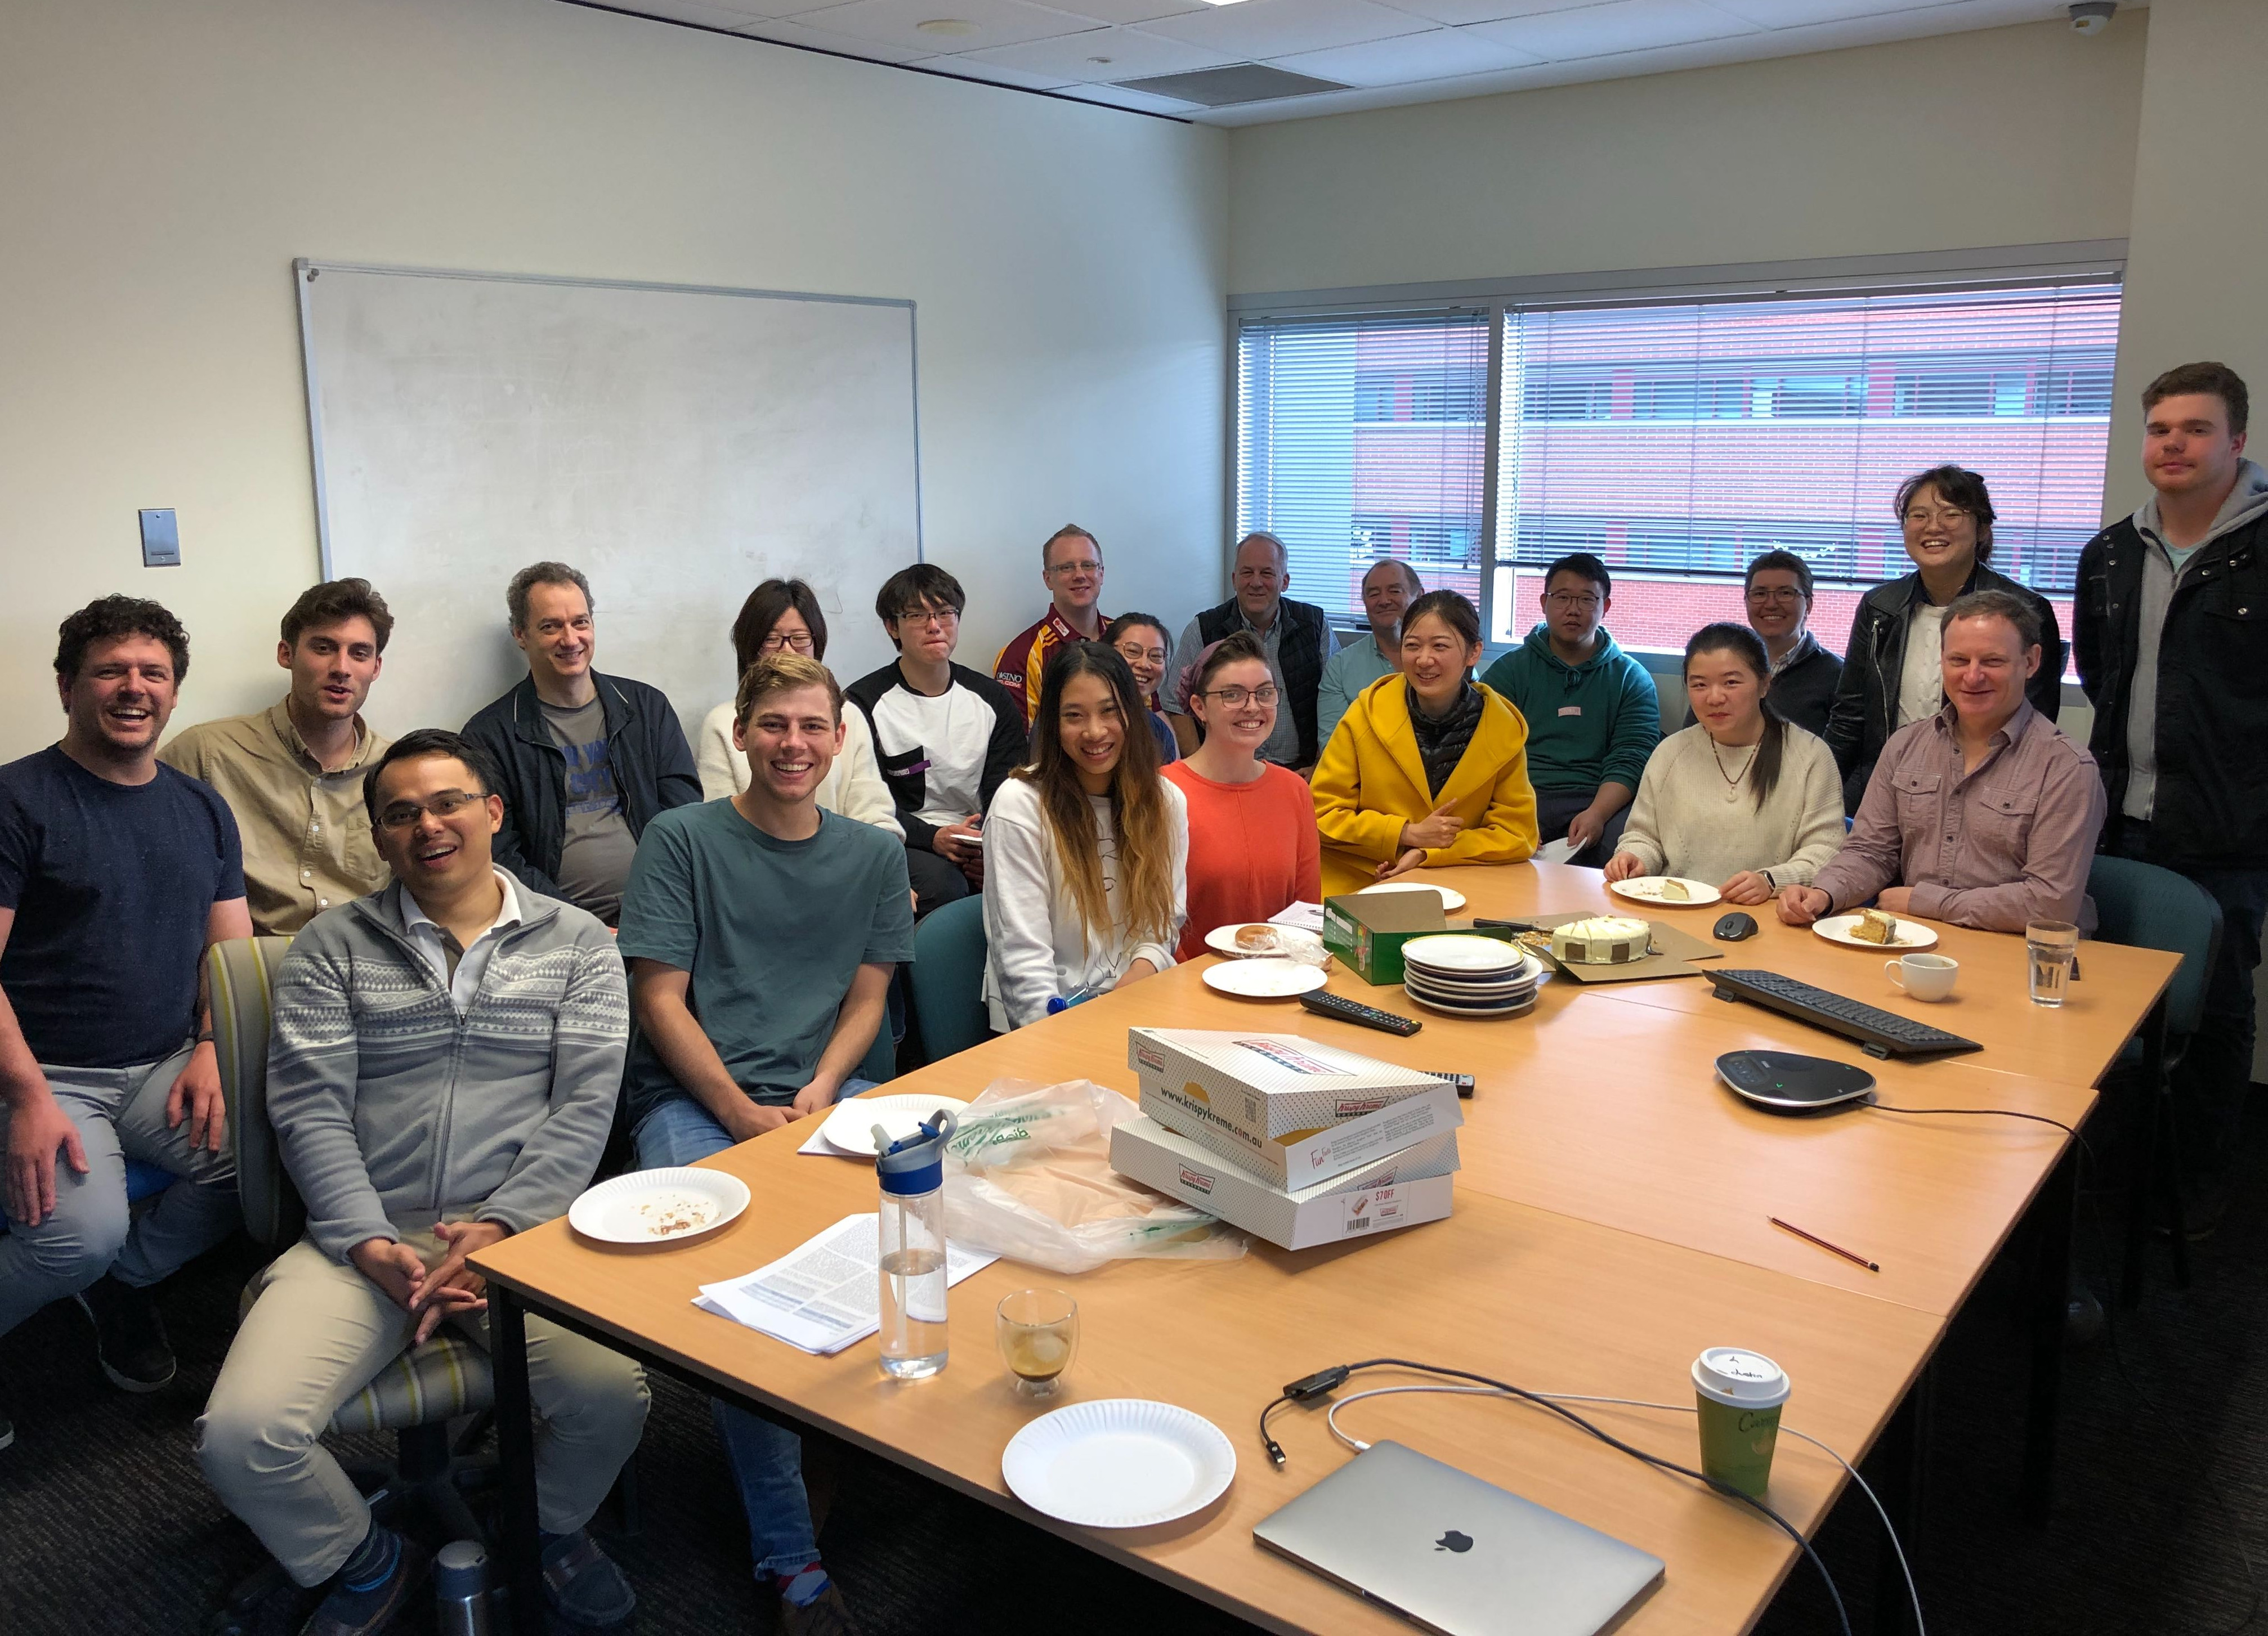
\includegraphics[width=0.75\linewidth]{figures/HubMeetingRoom.jpg}\\
\textit{Journal Club on Steve's Birthday, 2019}\\[1cm]

\end{frame}

\begin{frame}{Publication Highlights}

\center

\includegraphics[width=0.7\linewidth]{figures/Nature.jpg} \\[1cm]

\end{frame}

\begin{frame}{Publication Highlights}

\center
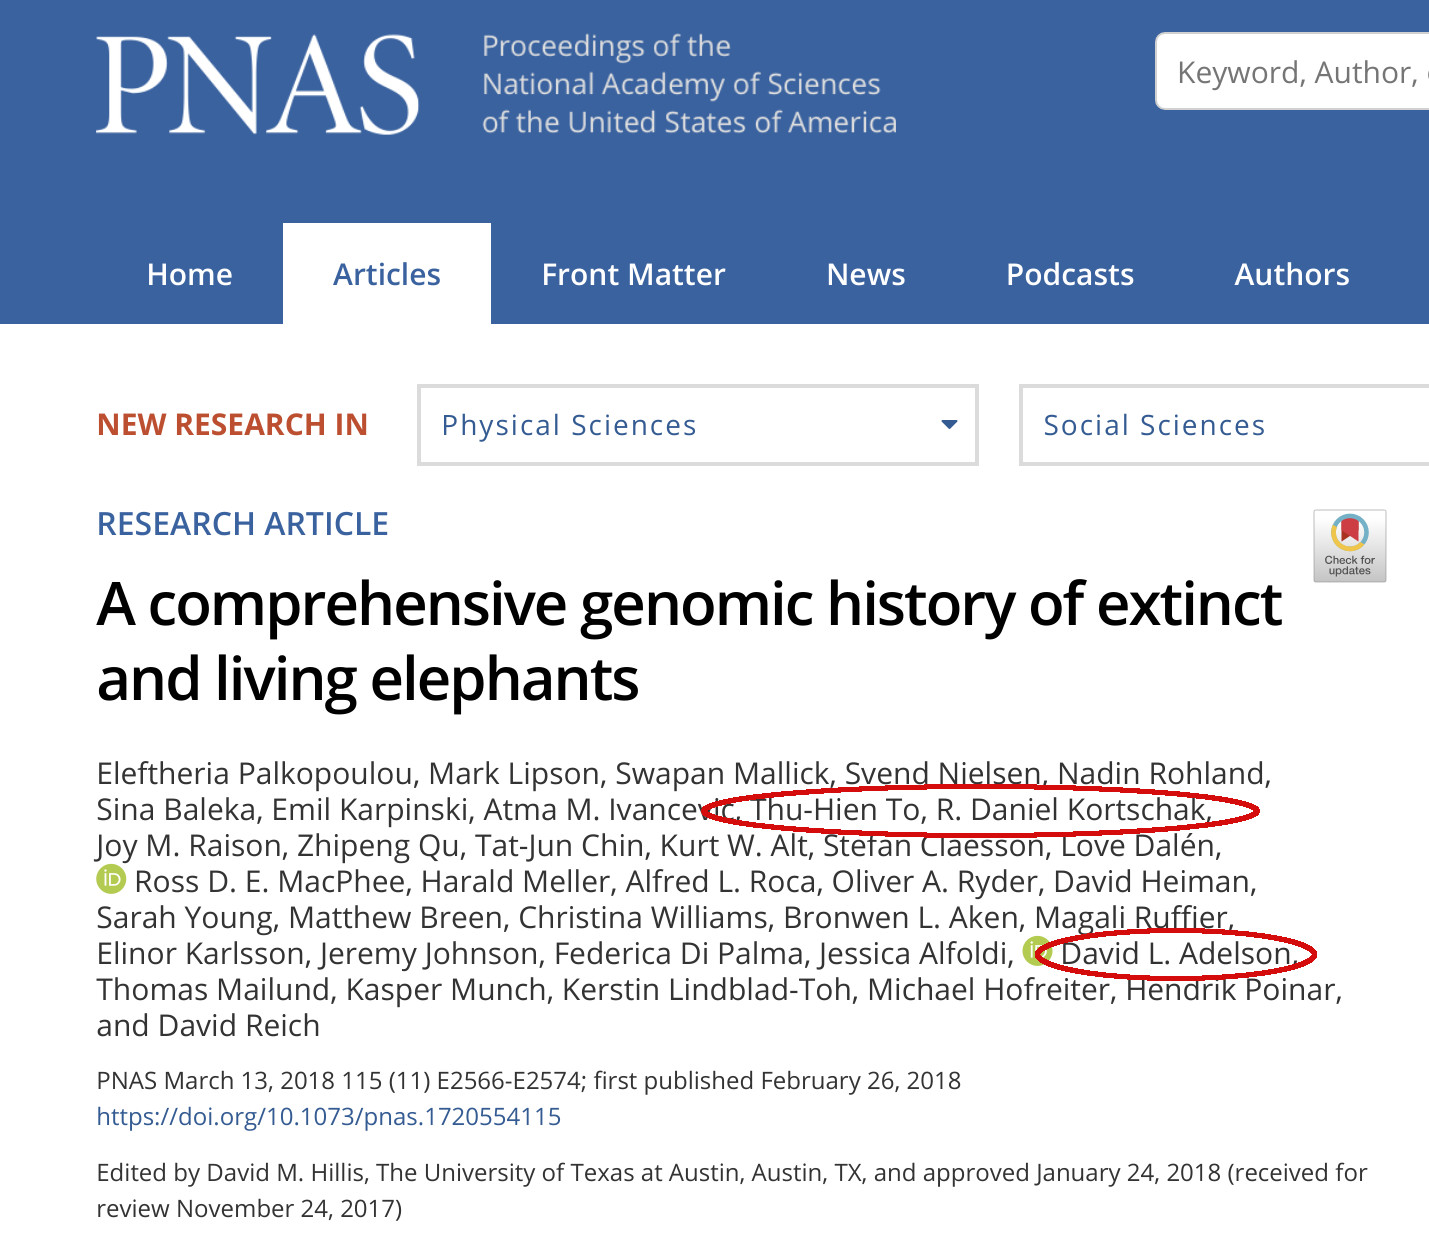
\includegraphics[width=0.7\linewidth]{figures/PNAS.jpg} \\[1cm]

\end{frame}


\begin{frame}{Other Highlights}

	\begin{itemize}
		\item Return on Investment over 6.5 years: \$4.4/dollar
		\item Improved PhD Completion rates (ECMS, Sciences, HMS)
		\begin{itemize}
			\item 66\% with no Hub engagement vs 75\% with ($p = 0.0091$)
		\end{itemize}	
		\item Establishment of UoA as a national player in bioinformatics
		\item Student engagements strongly biased towards women:
		\begin{itemize}
			\item ECMS: 41.7\% Vs 22.0\% (12 students)
			\item HMS: 61.9\% Vs 59.5\% (89 students)
			\item Sciences: 59.2\% Vs 48.3\% (260 students)\\[1cm]
		\end{itemize}
	\end{itemize}

\end{frame}

\begin{frame}{Weaknesses}

	\begin{itemize}
		\item Strategic Vision authored and submitted to Exec Dean of Sciences in 2018
		\item Rejected in it's entirety with no further discussion
		\item Included reimbursement for teaching courses
		\item In 2019 he approved a separate bioinformatics position inside School of BS (still unappointed)\\[1cm]

	\end{itemize}

\end{frame}

\begin{frame}{Weaknesses}

	\begin{itemize}
		\item Income
		\begin{itemize}
			\item Money from grants awarded
			\item Money for course delivery \& student supervision
		\end{itemize}		 
		\item No expectation of reimbursement from DVCR
		\item Short-term contracts made leading grant applications challenging
		\begin{itemize}
			\item I'm too junior
		\end{itemize}
		\item Lack of single ``high-profile" project
		\item How to limit access whilst providing open-access?\\[1cm]
	\end{itemize}

\end{frame}

\begin{frame}{Challenges}

In 6.3 years

	\begin{itemize}
		\item Biological Sciences: 4 Heads of School
		\item Agriculture, Food \& Wine: 4 Heads of School	
	\end{itemize}

\end{frame}

\begin{frame}{SAGC / Our Demise}

	\begin{itemize}
		\item Current DVCR didn't believe he should fund us
		\begin{itemize}
			\item Gave additional money to faculties for these projects
			\item HMS unambiguously supportive whilst Sciences ``receive no benefit at all from the Bioinformatics Hub"\blfootnote{As told to me by The Office of DVCR}
			\item Sciences subsequent internal review found we were beneficial \& vital infrastructure requiring funding
		\end{itemize}
		\item 3 positions provided by UofA as ``in-kind" for SAGC funding 
		\begin{itemize}
			\item 1xDVCR, 1xHMS, 1xSciences
			\item DVCR re-negotiated this down to the HMS position only\\[5mm]
		\end{itemize}
	\end{itemize}

\end{frame}

\begin{frame}{My role}

	\begin{itemize}
		\item I was ready to move on this year
%		\begin{itemize}
%			\item Offered a position at SVI developing scRNA methods
%			\item (The week after state borders closed $\ldots$)
%		\end{itemize}
		\item There was a position explicitly for me at SAGC
		\item Being spread across literally everything is exhausting
		\item Being funded on the whims of DVCR, Exec Deans etc is not ideal
		\item Looking to focus more deeply both \textit{biologically} and \textit{bioinformatically}
		\item Take full advantage of my ``ECR window"
	\end{itemize}

\end{frame}


\section{Enrichment Analysis}

\begin{frame}{RNA Seq Data}

	\begin{itemize}
		\item RNA Seq data can suffer from multiple biases
		\begin{itemize}
			\item Longer genes will produce more reads $\implies$ higher expression
			\item Higher expression $\implies$ more chance of being detected as DE
		\end{itemize}
		\item Can also suffer from GC bias (PCR)
		\item Conventionally assumed these factors are constant across samples
	\end{itemize}

\end{frame}

\begin{frame}{Enrichment Testing}
	\begin{itemize}
		\item Two primary types of enrichment testing
		\begin{enumerate}
			\item Enrichment within one set of genes (DE) compared to another set of genes (not DE)
			\item Ranked-list based approaches
		\end{enumerate}
		\item Both can be susceptible to GC, length or other biases
	\end{itemize}
\end{frame}

\subsection{Enrichment within DE genes}

\begin{frame}{Fisher's Exact Test}

	\begin{table}[ht]
	\centering
	\small
	\begin{tabular}{lrr}
		\toprule
		\textbf{Gene-set} & \textbf{Not DE} & \textbf{DE} \\ 
		\midrule
		Non-coding & 623 &  13 \\ 
		Protein Coding & 9670 & 378 \\ 
		\midrule
		(Totals) & 10293 & 391\\
	   \bottomrule
	\end{tabular}
	\end{table}
	
	\begin{itemize}
		\item Is the proportion of genes in our gene set higher in DE vs Not DE?
		\item We use Fisher's Exact Test (Hypergeometric Distribution)
	\end{itemize}
	
\end{frame}
	
\begin{frame}{Fisher's Exact Test}	

	\begin{table}[ht]
	\centering
	\small
	\begin{tabular}{lrr}
		\toprule
		\textbf{Gene-set} & \textbf{Not DE} & \textbf{DE} \\ 
		\midrule
		Non-coding & 623 &  13 \\ 
		Protein Coding & 9670 & 378 \\ 
		\midrule
		(Totals) & 10293 & 391\\
	   \bottomrule
	\end{tabular}
	\end{table}

	\begin{itemize}
		\item We would expect $\frac{9670}{10293} \times 391 = 0.940 \times 391 = 367$
		\item Significantly greater than this would be considered enrichment
		\item Fisher's Exact Test gives $p = 0.02$
	\end{itemize}
	
\end{frame}

\begin{frame}{Fisher's Exact Test}
	\begin{itemize}
		\item Fisher's Exact Test assumes equal probability of sampling each gene
		\item If we have bias in our sampling $\implies$ spurious results
		\item We can imagine the probability of sampling red or blue balls from a bag
		\item If balls are different sizes, we would have sampling bias
		\item \textit{Does gene length impact the probability of a gene being DE?}
	\end{itemize}
\end{frame}

\begin{frame}{Sampling Bias}
		
	\centering
	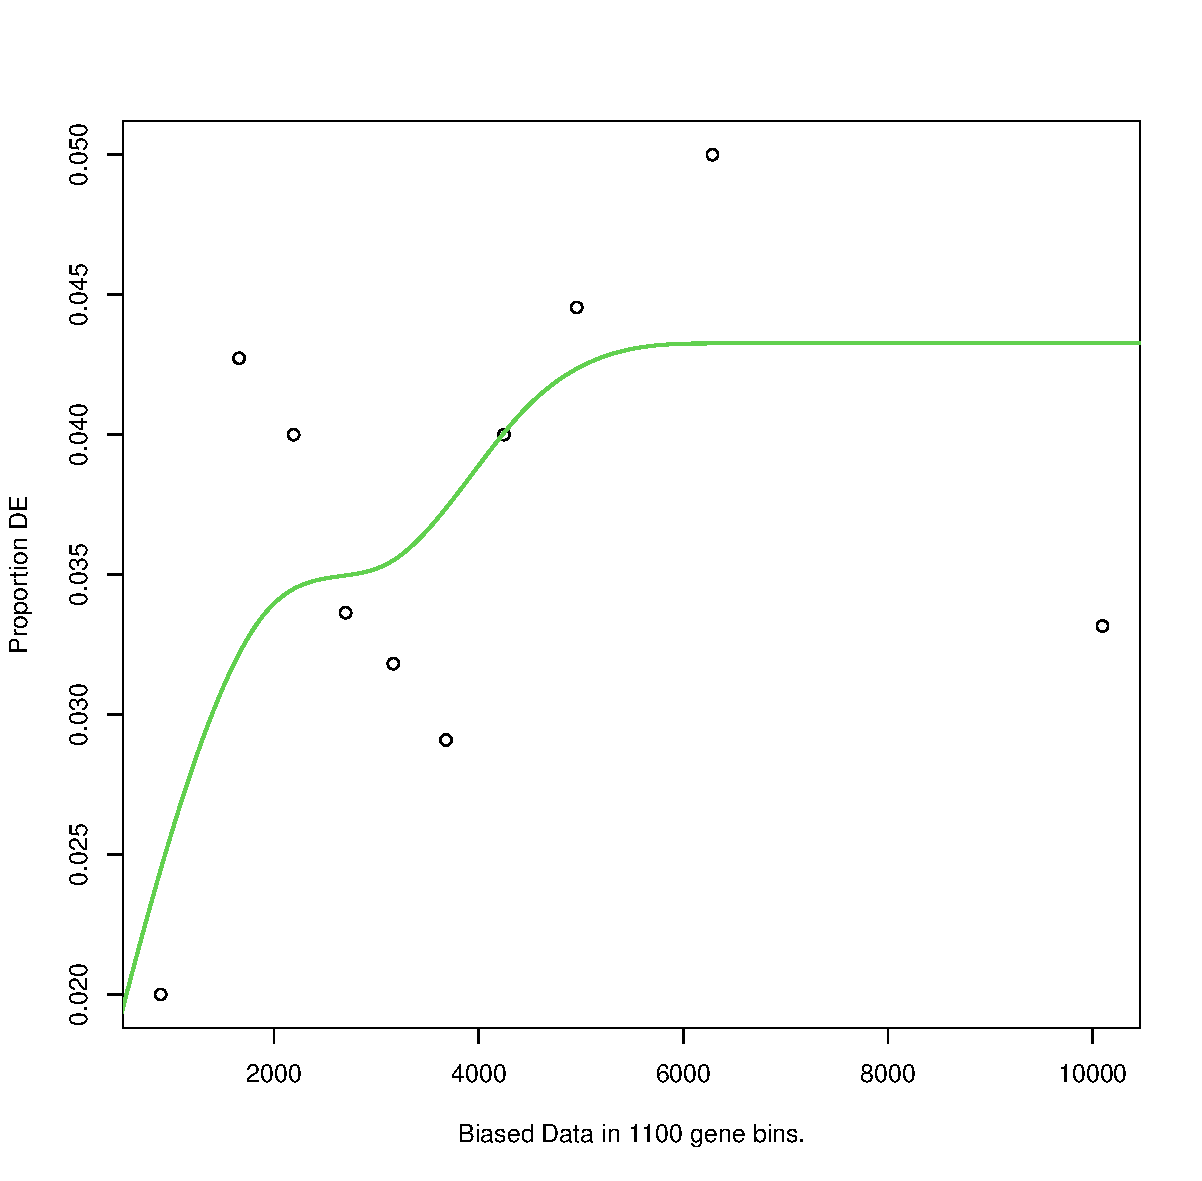
\includegraphics[width=0.5\linewidth]{figures/SamplingBias.pdf} \\
	Shorter genes appear less likely to be DE\\[5mm]

\end{frame}

\begin{frame}{Sampling Bias}

	\begin{itemize}
		\item Wallenius’ Non-Central Hypergeometric Distribution allows for sampling with bias
		\item Implemented in the package \texttt{goseq}
		\item Given that shorter genes are less likely to be DE for this dataset we should use this here
		\item For the same $2\times2$ table we get $p = 0.14$\\[5mm]
	\end{itemize}
	
\end{frame}

\begin{frame}{Sampling Bias}

Does it really matter?

	\begin{itemize}
		\item If dancing around $p \leq 0.05$, then \textit{yes}
		\item For enrichment testing, the best results are indisputible ($p \ll 0.05$) and for these, \textit{not so much}
	\end{itemize}		

\end{frame}

\subsection{Enrichment Using Ranked Lists}

\begin{frame}{Ranked List Approaches}

	\begin{itemize}
		\item Gene lists are ranked based on a statistic ($t$, $p$, logFC etc)
		\item Walking down the list detects any unexpected clustering of genes from a gene set at either end
	\end{itemize}
	
	\center
	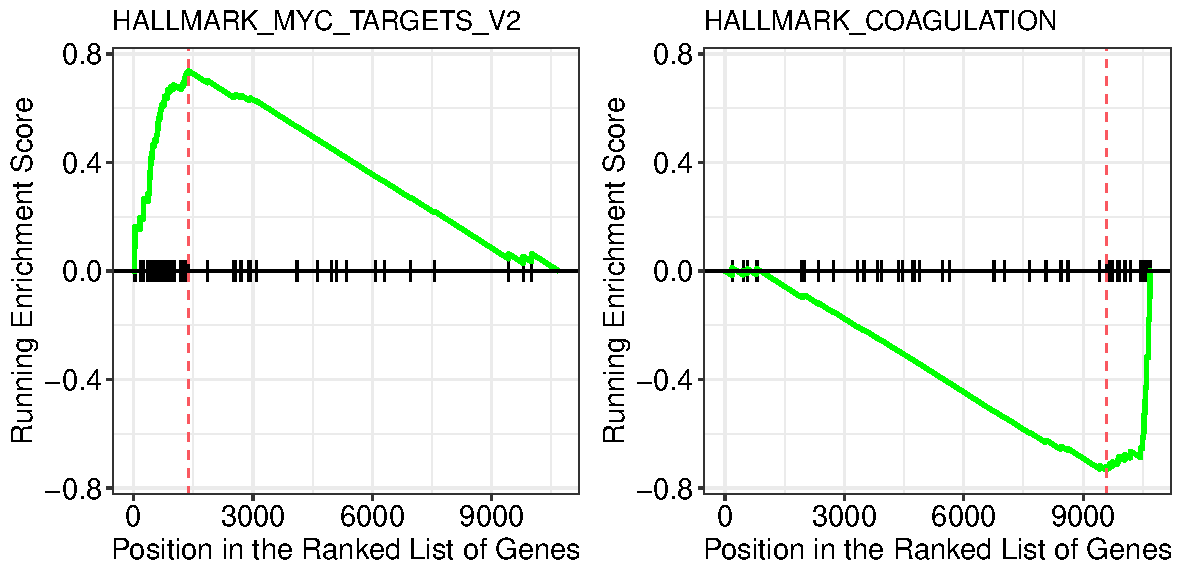
\includegraphics[width=0.7\linewidth]{figures/BarcodePlot.pdf} 

\end{frame}

\begin{frame}{GC and Length bias}

	\begin{itemize}
		\item Generally, GC \& length bias within a dataset was assumed to be trivial
		\item This has been shown to be violated more often than thought (\textit{\cite{MandelboumRNABias}})
		\item Can have non-trivial impacts when using ranked lists
	\end{itemize}

\end{frame}

\begin{frame}{GC and Length bias}

	\center
	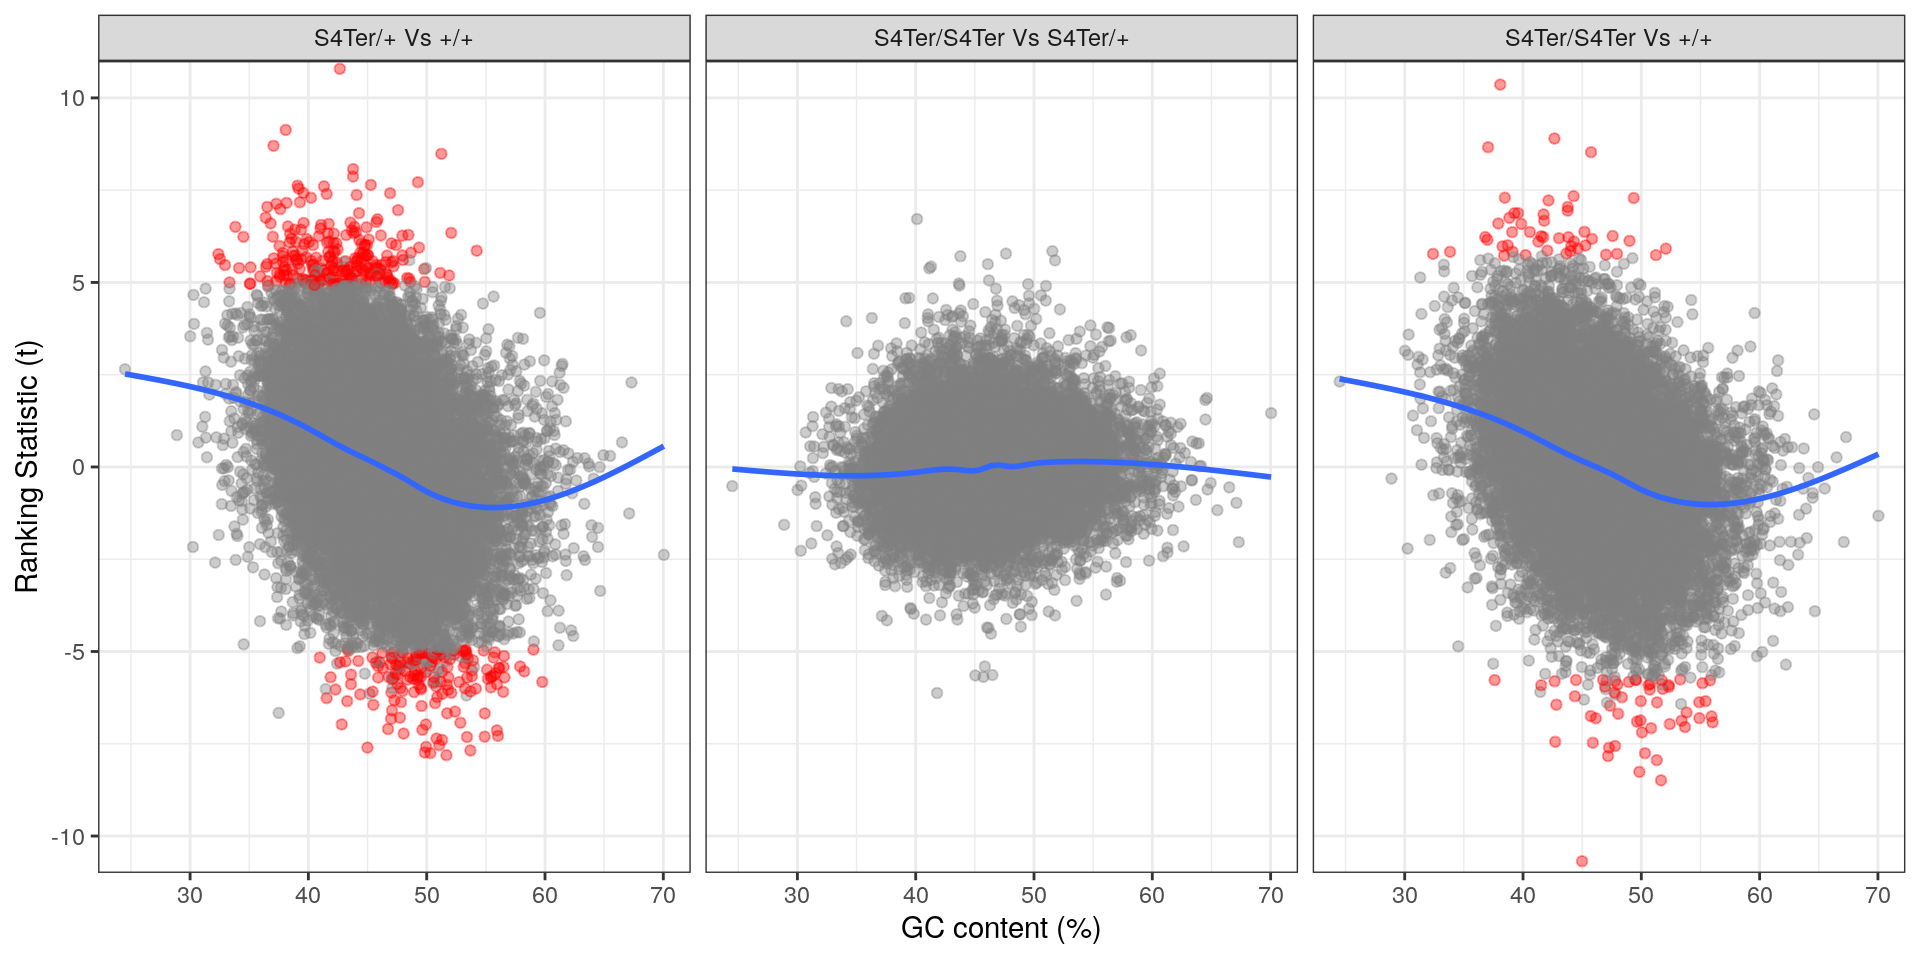
\includegraphics[width=0.9\linewidth]{figures/voomGCBias-1.png} \\
	Both Mutant vs WT comparisons have non-trivial GC issues\\[1cm]
	
\end{frame}

\begin{frame}{GC and Length bias}	

	\center
	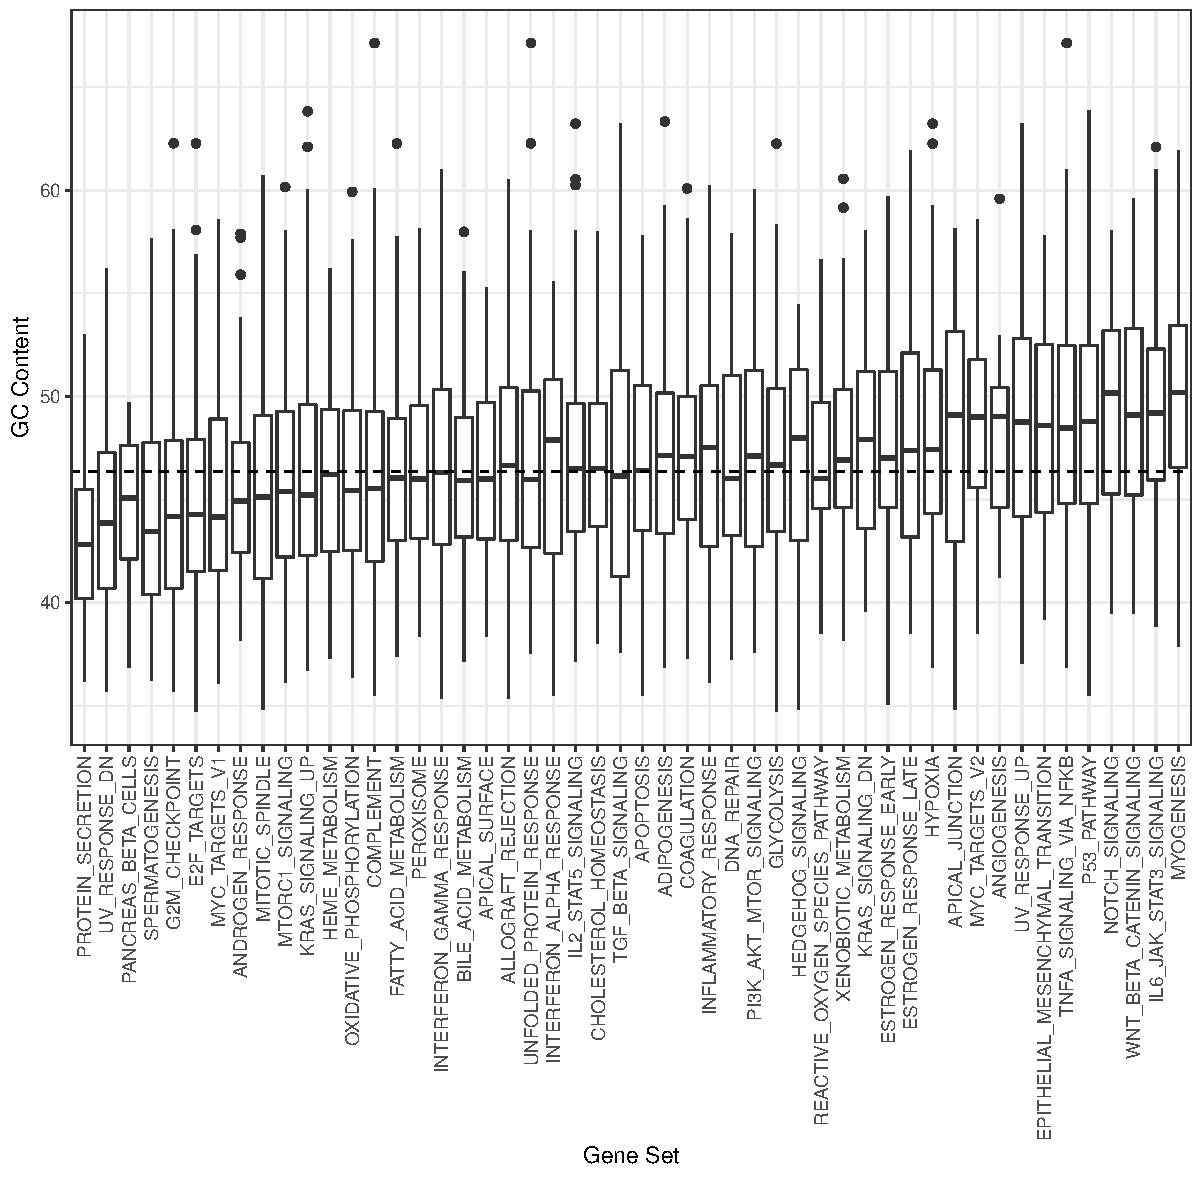
\includegraphics[width=0.65\linewidth]{figures/GeneSetGC.pdf} 

\end{frame}

\begin{frame}{Managing Bias}

	\begin{itemize}
		\item Conditional Quantile Normalisation (CQN) can mitigate this (unless extreme)
		\item Incorporates a gene and sample specific offset for length and GC bias
		\begin{itemize}
			\item Rules out \texttt{voom} $\implies$ Negative Binomial models only
		\end{itemize}
		\item TMM normalisation is fine for well-behaved data
	\end{itemize}

\end{frame}

\section{Incucyte Analysis}

\begin{frame}{Incucyte Data}

	\begin{itemize}
		\item Data from the Incucyte is challenging to \textit{analyse} and to \textit{visualise}
		\item Richard \& Jean asked for help in May
		\item Have a manual import R script running
		\item Have some viable code for visualisation
		\item Have some opaque code for fitting statistical models
	\end{itemize}

\end{frame}

\begin{frame}{Incucyte Data}

	\begin{itemize}
		\item Plan is to build an R package with:
		\begin{itemize}
			\item Easy data import
			\item Easy data visualisation
			\item Viable analytic approaches
		\end{itemize}
		\item Publish a workflow for visualisation and statistical analysis
	\end{itemize}

\end{frame}


\begin{frame}{Data Parsing}

	\begin{itemize}
		\item Code for parsing data works well
		\item Only parses count/intensity data
		\item Uses fancy text searching to extract groups and treatments
		\item Wrote a parser for the \texttt{*PlateMap} files over the weekend
		\item Plan to define an \texttt{R} object with metadata + intensities
	\end{itemize}

\end{frame}

\subsection{Data Visualisation}

\begin{frame}[fragile]{Data Visualisation}

	\begin{itemize}
		\item Current visualisation code works, but looks intimidating
		\item Plan is to write simple plotting functions on my object class
	\end{itemize}

%\end{frame}
%
%\begin{frame}{Data Visualisation}

	\begin{lstlisting}[language=R]
	plateMap <- parsePlateMap(f = "Vessel 897 T47D 2B Kate sytox caspase.PlateMap")
	plotPlateMap(plateMap) +
    	scale_fill_discrete(na.value = NA) +
	    theme_bw() +
	    theme(panel.grid = element_blank())
	\end{lstlisting}
	

\end{frame}

\begin{frame}[fragile]{Data Visualisation}

	\center
	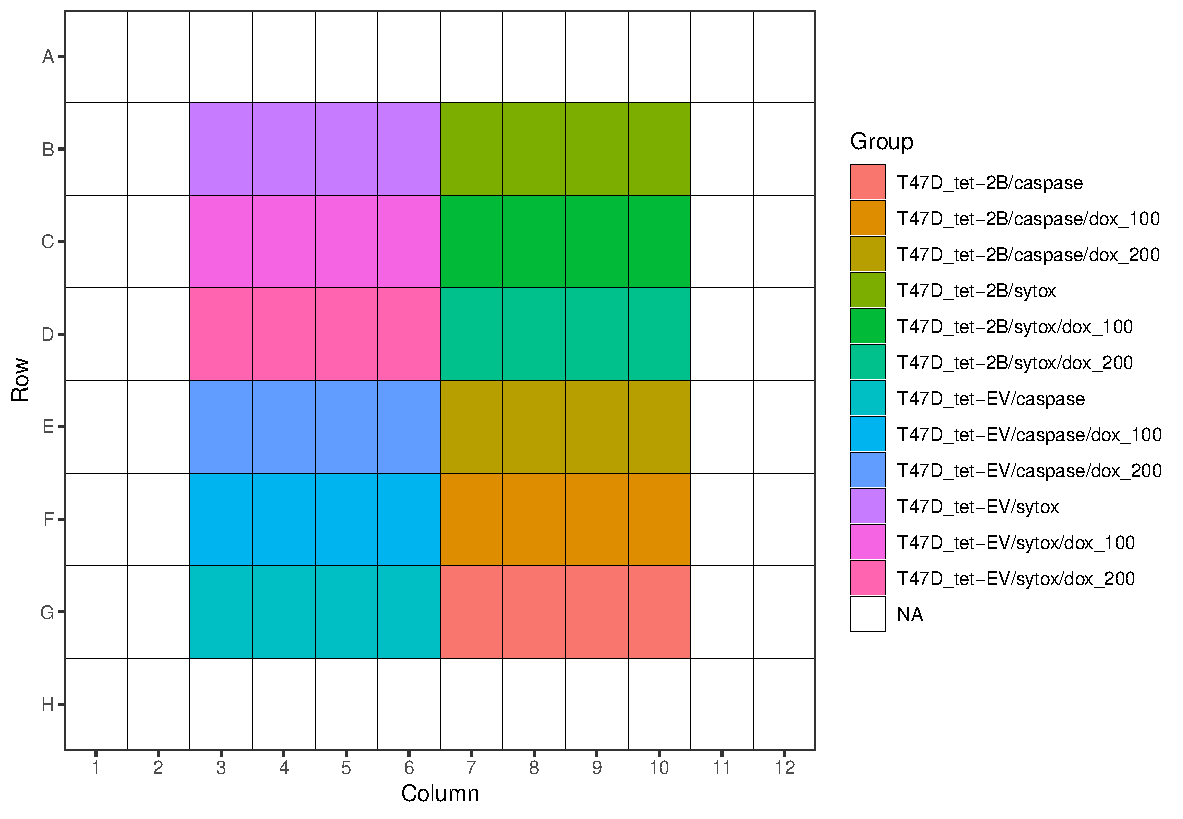
\includegraphics[width=0.8\linewidth]{figures/PlateMap.pdf} 


\end{frame}

\begin{frame}[fragile]{Data Visualisation}

	\center
	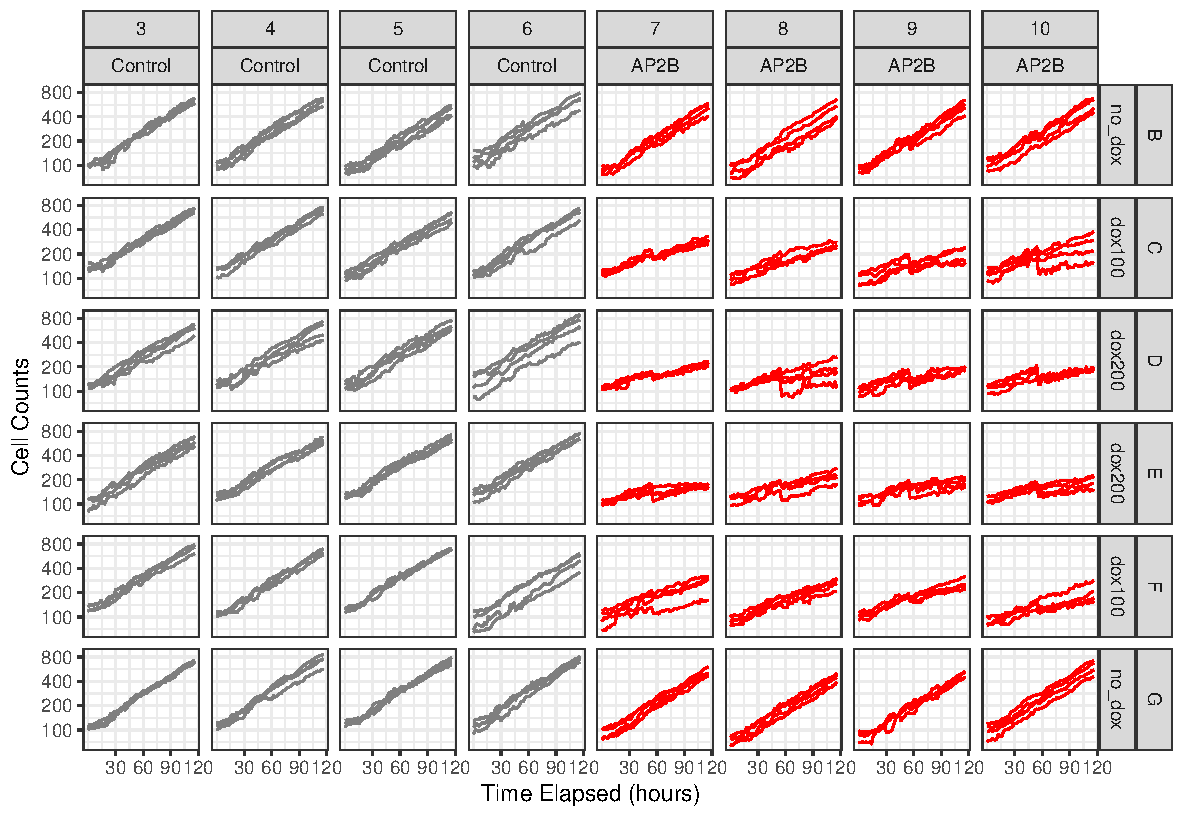
\includegraphics[width=0.75\linewidth]{figures/RawCurves.pdf} \\[5mm]

\end{frame}

\begin{frame}[fragile]{Data Visualisation}
	
	\center
	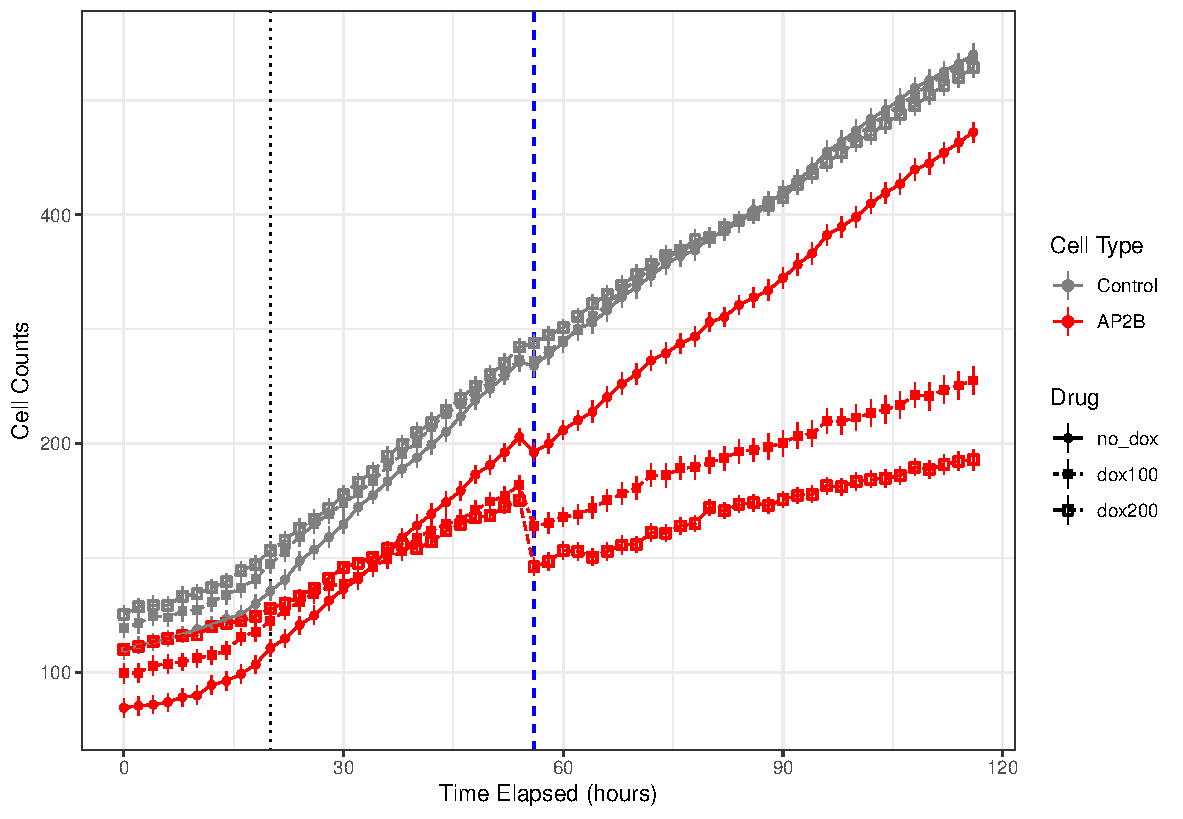
\includegraphics[width=0.75\linewidth]{figures/SummarisedCurves.pdf} \\[5mm]

\end{frame}

\subsection{Cell Growth}

\begin{frame}{Growth Data: Analytic Challenges}

	\begin{itemize}
		\item Cell counts are discrete $\implies$ Poisson distributed data
		\begin{itemize}
			\item This is a type of Generalised Linear Model (GLM)
			\item Poisson Distributions measure counts per unit of measurement
			\item The rate parameter ($\lambda$) models the number of counts/unit
			\item Here we have cells/image
		\end{itemize}
		\item Poisson models for the Incucyte will fit the
		\begin{enumerate}
			\item starting number of cells (i.e. the intercept) and,
			\item change in the rate of counts as a function of time (i.e. the slope)
		\end{enumerate}			
		\item Can be fit for each treatment group, or individual treatments
	\end{itemize}

\end{frame}

\begin{frame}{Growth Data: Analytic Challenges}

	\begin{itemize}
		\item Data is also captured within each image, within each well
		\begin{itemize}
			\item This introduces correlations within each image/well
			\item Leads to underestimate of standard errors
			\item Leads to overestimate of significance
		\end{itemize}
		\item A nested model should be applied
		\begin{itemize}
			\item Commonly known as \textit{mixed-effects models}
			\item Allows for random variability in \textit{intercepts} between images
			\item Potentially allows the same for slopes
		\end{itemize}
		\item End model is a Generalised Mixed-Effects Model
	\end{itemize}

\end{frame}

\begin{frame}{GLMMs}

	\begin{itemize}
		\item GLMMs are notoriously challenging
		\item To estimate model effects for a linear (Gaussian) model $\implies$ simple matrix algebra ($<1s$)
		\item To estimate effects for a GLMM:
		\begin{itemize}
			\item Fit model iteratively using EM-algorithm
			\item Can take minutes			
			\item Requires convergence to be considered valid
			\item Nesting of model terms within images can impede convergence
		\end{itemize}
	\end{itemize}
	
\end{frame}	

\subsection{Cell Death}
	
\begin{frame}{Cell Death: Analytic Challenges}

	\begin{itemize}
		\item Cell death is a function of cell growth
		\item e.g. 10 dead cells could be 10/10, or 10/1000
		\item Needs to analysed incorporating cell growth
		\item Cell growth counts are implicitly cumulative
		\item Cell death counts are transient
	\end{itemize}

\end{frame}

\begin{frame}{Cell Death: Analytic Challenges}

	\begin{itemize}
		\item Do we analyse two cumulative variables?
		\item Do we analyse two transient variables?
		\item Do we just take a time-point as a snapshot and ignore this?
	\end{itemize}
	
	
\end{frame}

\begin{frame}{Cell Death: Analytic Challenges}

	\center
	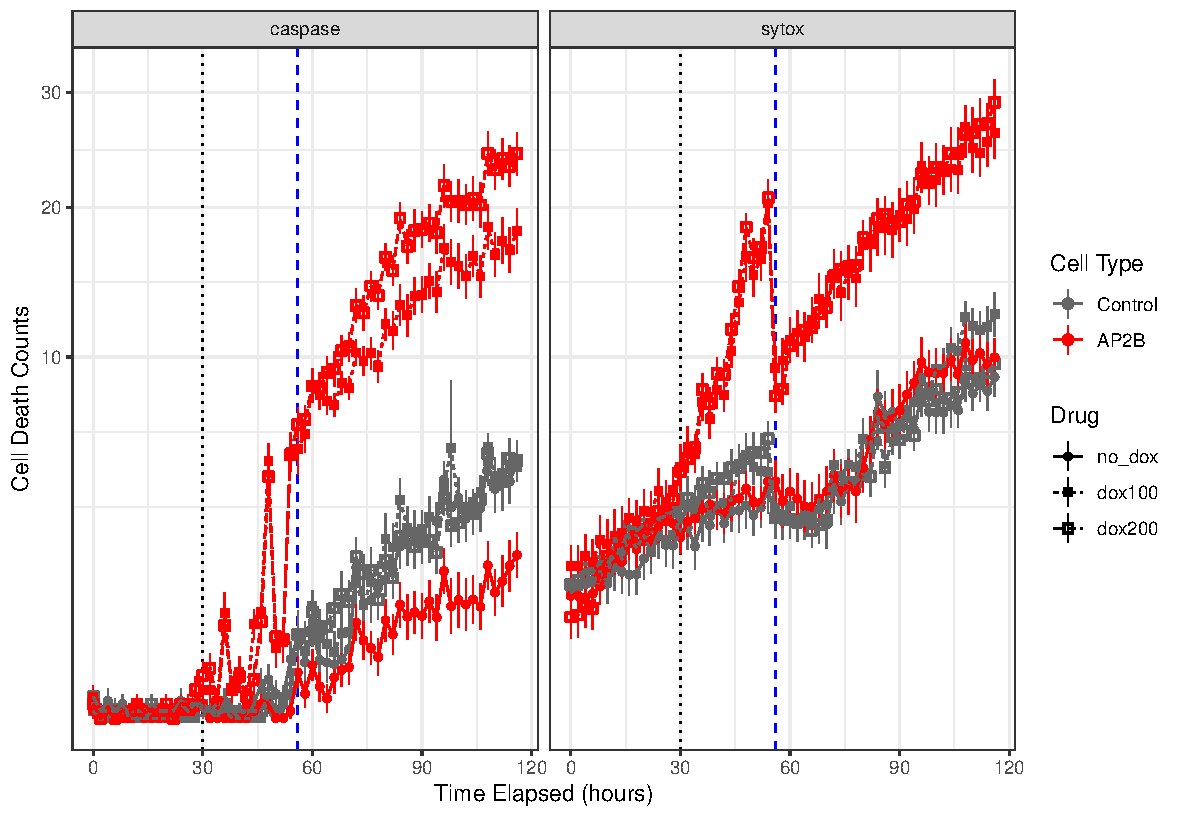
\includegraphics[width=0.75\linewidth]{figures/DeathCounts.pdf} 

\end{frame}

\begin{frame}{Cell Death: Analytic Challenges}

	\center
	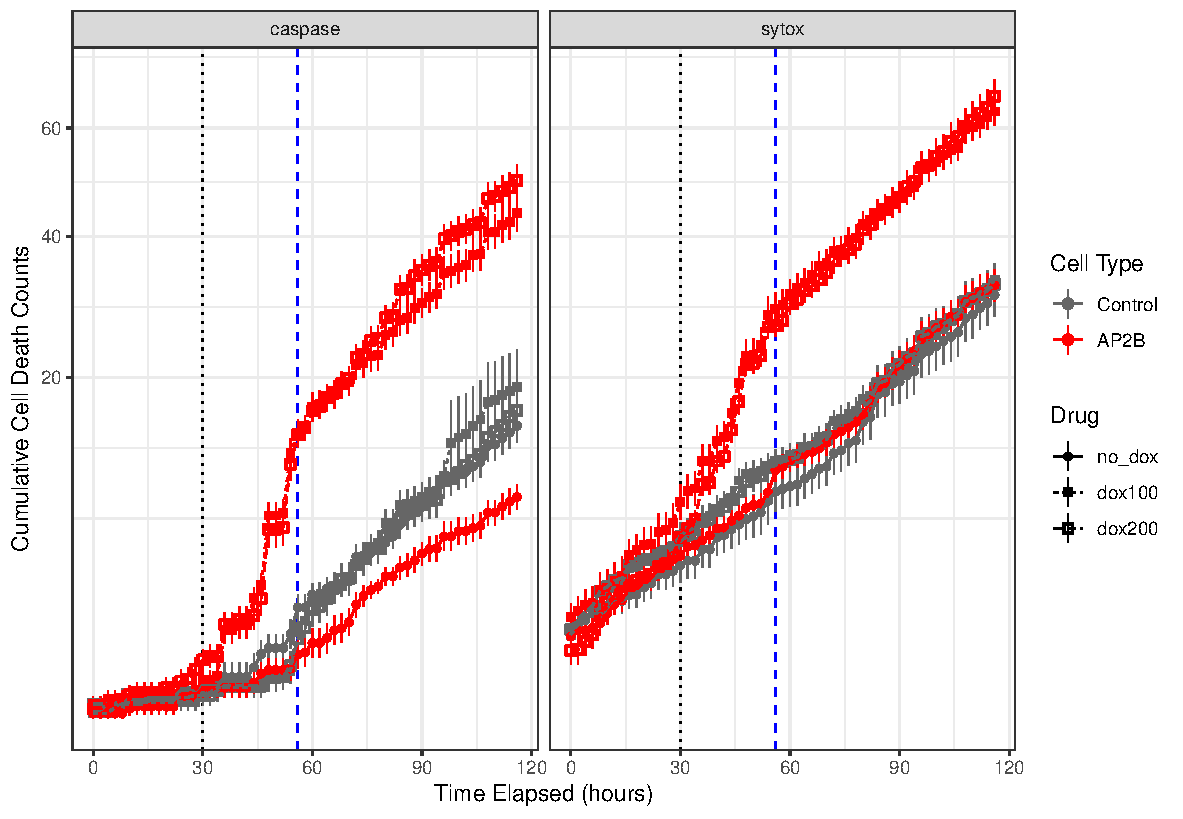
\includegraphics[width=0.75\linewidth]{figures/CumulativeDeathCounts.pdf} 

\end{frame}

\begin{frame}{Cell Death: Analytic Challenges}

	\begin{itemize}
		\item Data looks like zero-inflated, binomial (i.e. logistic) regression
		\begin{enumerate}
			\item First we find the probability of observing $>0$ dead cells with time
			\item Then we fit the proportion of dead cells 
		\end{enumerate}
		\item This models the probability of a binary outcome, e.g. death = success
		\item Could fit:
		\begin{enumerate}
			\item The proportion of dead cells at time $t$ (transient)
			\item The total proportion of cells that have died by time $t$ (cumulative)
		\end{enumerate}
	\end{itemize}
	
\end{frame}

\begin{frame}{Probability of Any Death}

	\center
	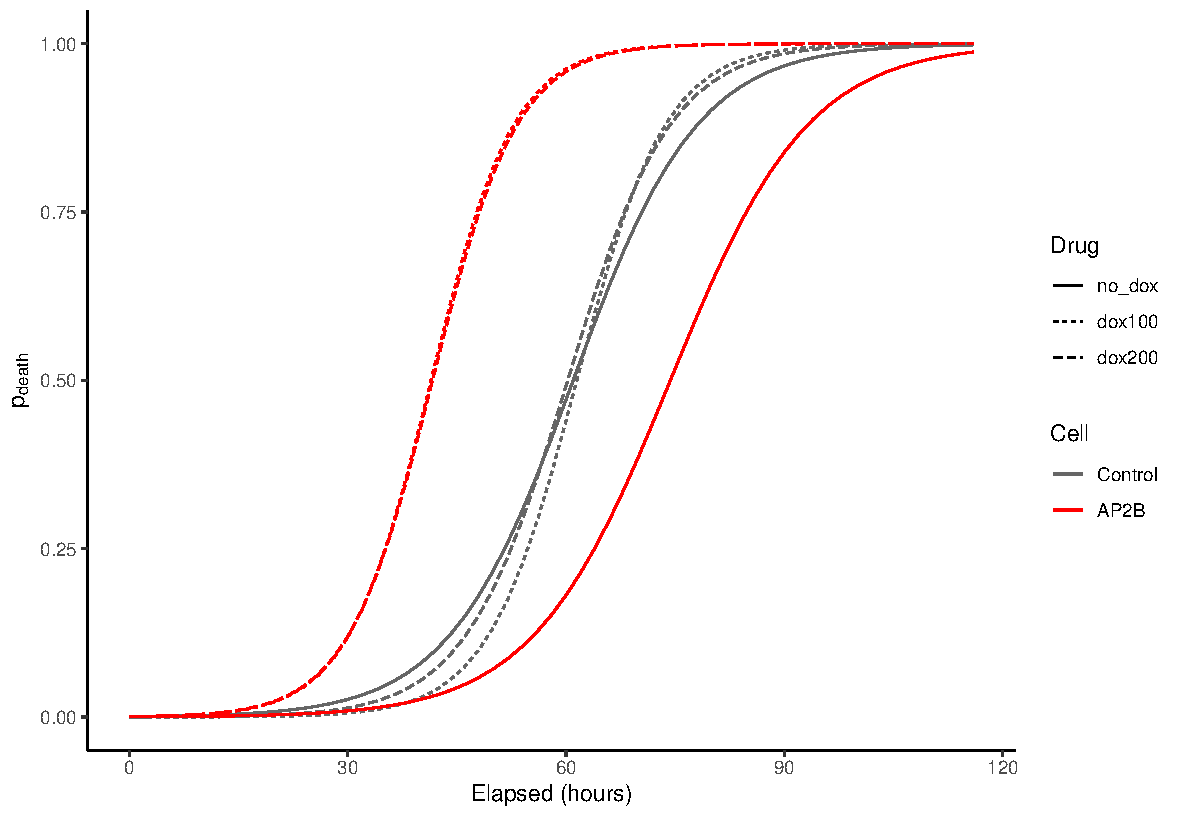
\includegraphics[width=0.75\linewidth]{figures/zeroMod.pdf} 	

\end{frame}

\begin{frame}{Proportion Dead (Transient)}

	\center
	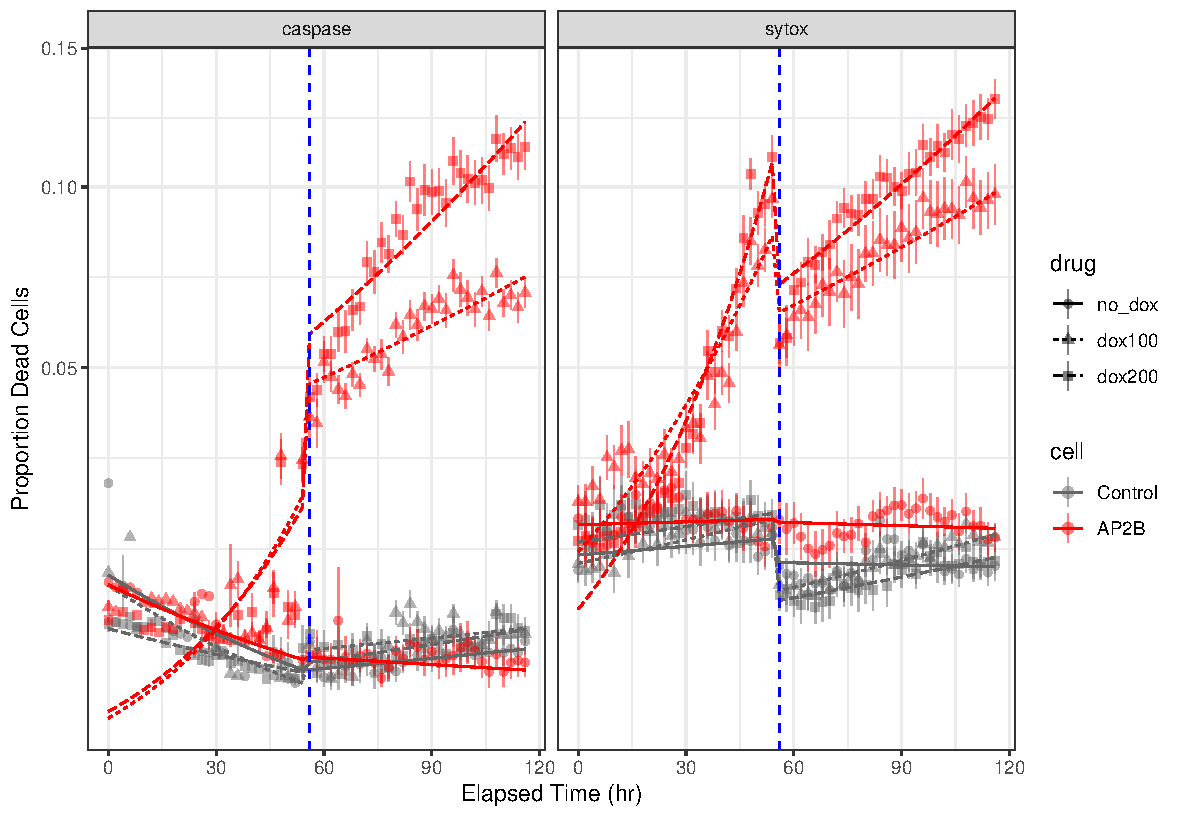
\includegraphics[width=0.75\linewidth]{figures/PropDead.pdf} 	

\end{frame}

\begin{frame}{Proportion Dead (Cumulative)}

	\center
	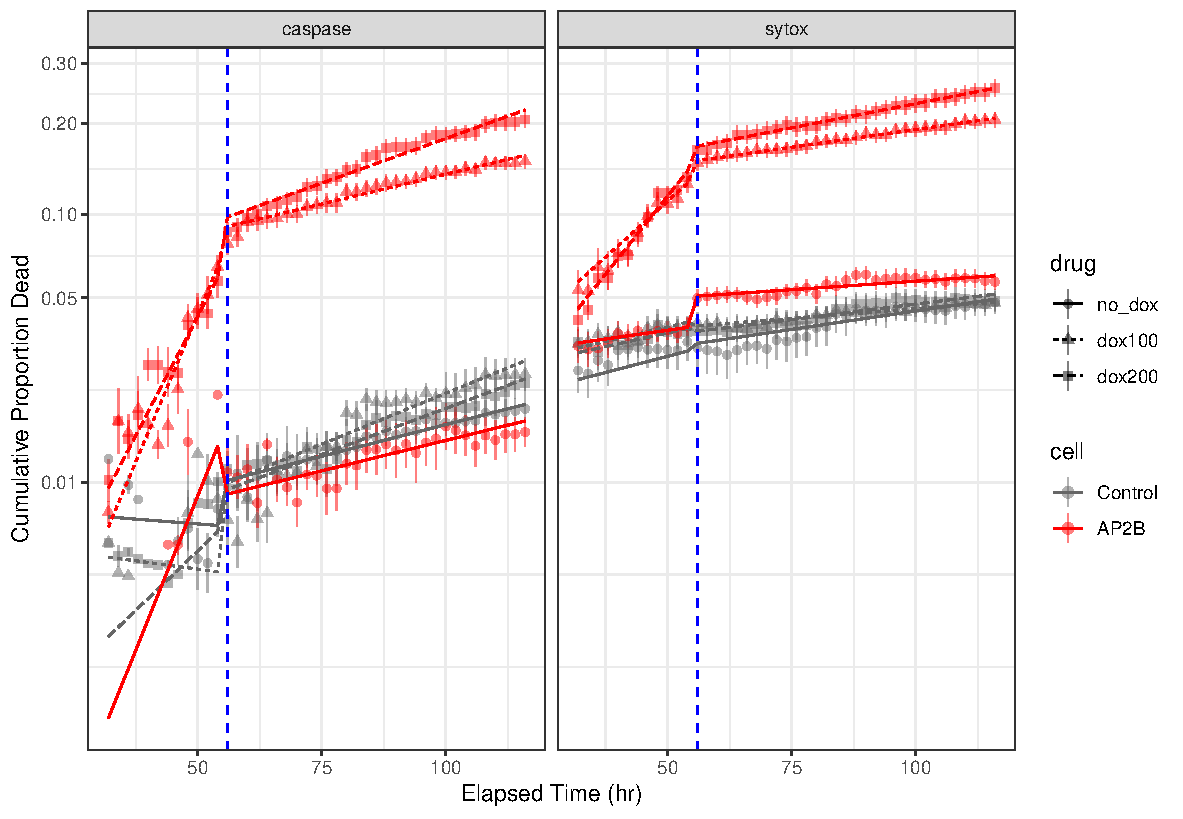
\includegraphics[width=0.75\linewidth]{figures/CumPropDead.pdf} 	

\end{frame}

\begin{frame}{Cell Death: Analytic Challenges}

	\begin{itemize}
		\item Comparison of slopes between groups is \textit{not appropriate}
		\item Need to analyse the differences in proportion dead
		\begin{itemize}
			\item Odds Ratio as a function of time?
		\end{itemize}
		\item This is sampling without replacement $\implies$ Hypergeometric, not Binomial (???)
		\item GLMM convergence issues remain solvable, but delicately balanced
	\end{itemize}

\end{frame}

\end{document}